\documentclass[tikz]{standalone}
\usepackage{pgfplots}
\begin{document}


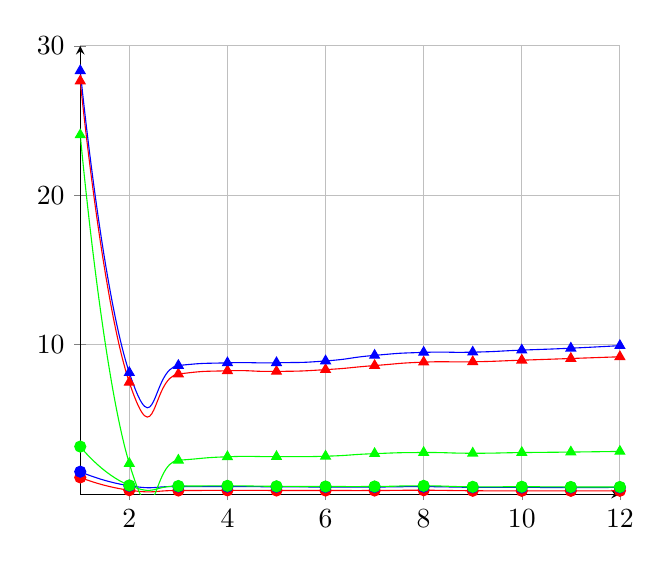
\begin{tikzpicture}
\begin{axis}[axis lines=middle, grid=both, ymin=0, ymax=30]\addplot [red, smooth, tension=1, mark=*] coordinates {(1, 1.118)(2, 0.262)(3, 0.242)(4, 0.254)(5, 0.245)(6, 0.242)(7, 0.241)(8, 0.259)(9, 0.226)(10, 0.222)(11, 0.221)(12, 0.223)};
\addplot [blue, smooth, tension=1, mark=*] coordinates {(1, 1.502)(2, 0.559)(3, 0.511)(4, 0.507)(5, 0.492)(6, 0.477)(7, 0.476)(8, 0.501)(9, 0.456)(10, 0.449)(11, 0.446)(12, 0.448)};
\addplot [green, smooth, tension=1, mark=*] coordinates {(1, 3.183)(2, 0.583)(3, 0.542)(4, 0.556)(5, 0.523)(6, 0.511)(7, 0.512)(8, 0.554)(9, 0.489)(10, 0.494)(11, 0.479)(12, 0.478)};
\addplot [red, smooth, tension=1, mark=triangle*] coordinates {(1, 27.647)(2, 7.481)(3, 8.038)(4, 8.253)(5, 8.212)(6, 8.33)(7, 8.603)(8, 8.832)(9, 8.855)(10, 8.963)(11, 9.076)(12, 9.192)};
\addplot [blue, smooth, tension=1, mark=triangle*] coordinates {(1, 28.332)(2, 8.13)(3, 8.607)(4, 8.786)(5, 8.791)(6, 8.912)(7, 9.285)(8, 9.485)(9, 9.5)(10, 9.636)(11, 9.766)(12, 9.938)};
\addplot [green, smooth, tension=1, mark=triangle*] coordinates {(1, 24.038)(2, 2.049)(3, 2.268)(4, 2.5)(5, 2.509)(6, 2.537)(7, 2.709)(8, 2.784)(9, 2.737)(10, 2.781)(11, 2.815)(12, 2.858)};
\end{axis}
\end{tikzpicture}
\end{document}